
\documentclass[tikz]{standalone}
\definecolor{DarkBlue}{rgb}{0,0,0.5} % 添加缺失的颜色定义
\begin{document}

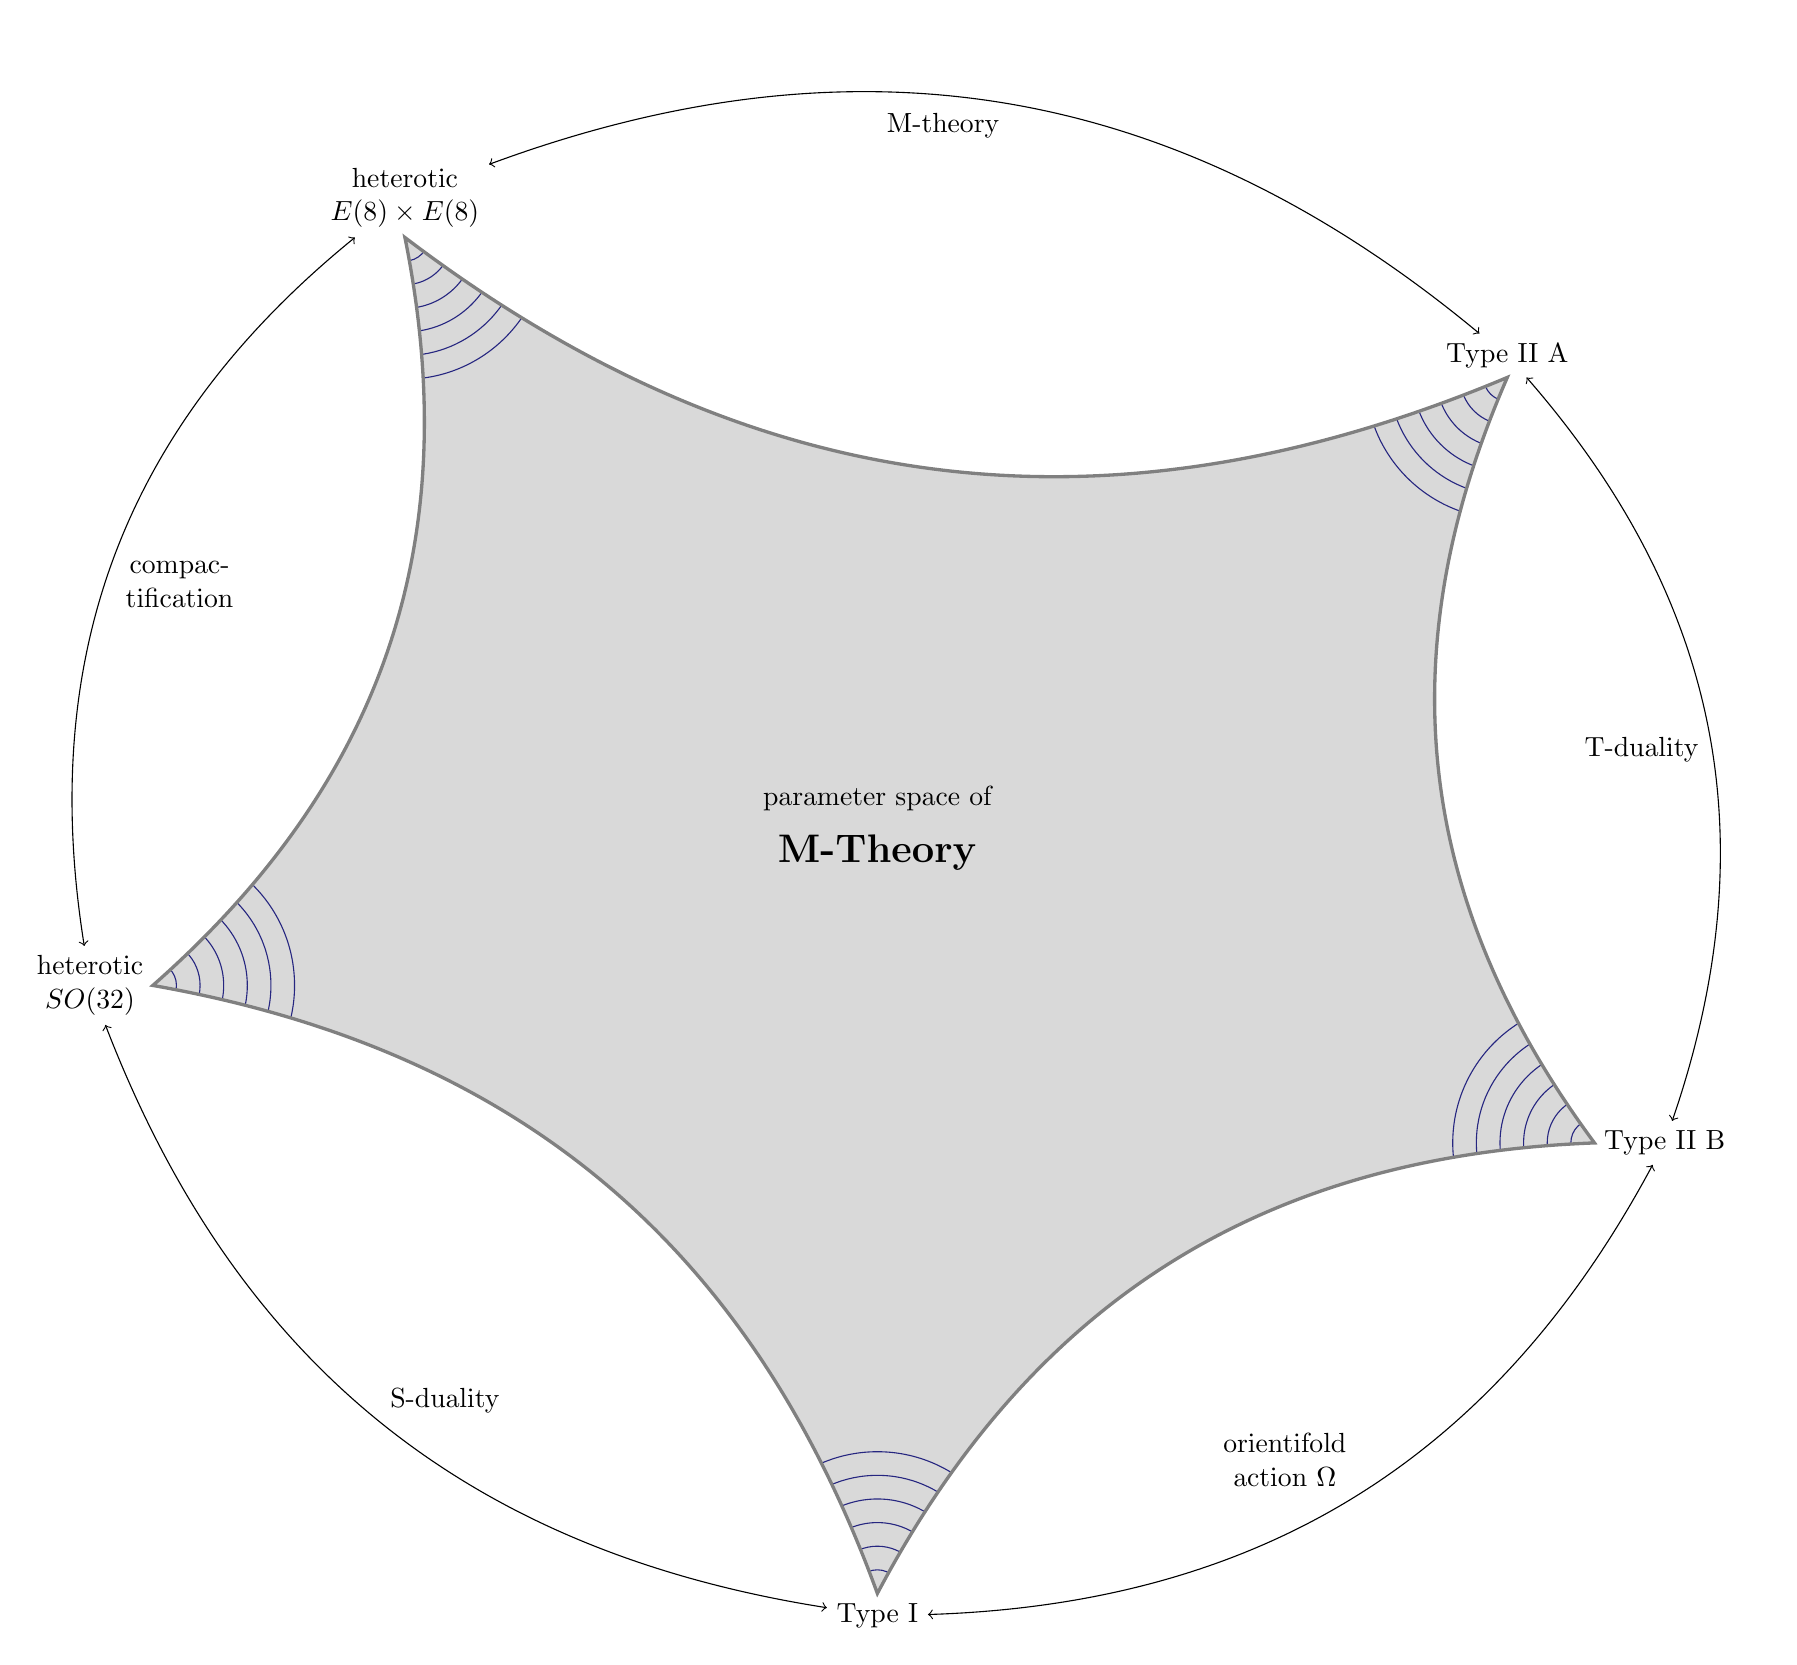
\begin{tikzpicture}[scale=2]
  \node (so32) [align=center] at (-5,-1) {heterotic\\$SO(32)$};
  \node (e8e8) [align=center] at (-3,4) {heterotic\\$E(8) \times E(8)$};
  \node (tiia) [align=center] at (4,3) {Type II A};
  \node (tiib) [align=center] at (5,-2) {Type II B};
  \node (ti) [align=center] at (0,-5) {Type I};

  \draw[bend left,<->] (so32) to node [below right,align=center] {compac-\\tification} (e8e8);
  \draw[bend left,<->] (e8e8) to node [below left] {M-theory} (tiia);
  \draw[bend left,<->] (tiia) to node [below left] {T-duality} (tiib);
  \draw[bend left,<->] (tiib) to node [above left,align=center] {orientifold\\action $\Omega$} (ti);
  \draw[bend left,<->] (ti) to node [above right] {S-duality} (so32);

  \begin{scope}
    % 修正路径绘制方式
    \clip (so32.east) to [bend right] (e8e8.south)
      to [bend right] (tiia.south)
      to [bend right] (tiib.west)
      to [bend right] (ti.north)
      to [bend right] cycle; % 闭合路径
    
    \foreach \c in {so32.east,e8e8.south,tiia.south,tiib.west,ti.north}{%
        \foreach \r in {1,...,6}{%
            \draw[DarkBlue] (\c) circle (\r*0.15cm); % 使用已定义的颜色
          }
      }
  \end{scope}

  % 修正路径绘制方式
  \draw[bend right,very thick,gray,fill,fill opacity=0.3] 
    (so32.east) to [bend right] (e8e8.south)
    to [bend right] (tiia.south)
    to [bend right] (tiib.west)
    to [bend right] (ti.north)
    to [bend right] cycle; % 闭合路径

  \node (mth) [align=center] at (0,0) {parameter space of\\[2ex]{\Large \textbf{M-Theory}}};
\end{tikzpicture}
\end{document}
